\documentclass[]{beamer}
\mode<presentation>{
  %% \usetheme[compress]{Berlin}
}
%% packages
\usepackage{zhspacing}
\zhspacing
\usepackage{graphics}
\usepackage{listings}
\lstset{basicstyle=\ttfamily\small}
\usepackage{tabularx}
\usepackage{booktabs}
%% meta info
\title{函数式并行程序语言研究}
\title{Writing Clang Tools}
\subtitle{An Introduction}
\author[SuXing~pysuxing@gmail.com]{SuXing}
\institute{TOW}
\date{\today}

%% slides
\begin{document}
\setlength{\parindent}{0pt}

\frame{\titlepage}

\frame{\tableofcontents}

\section{Clang AST}
\frame{\tableofcontents[currentsection]}
\begin{frame}
  \frametitle{Overview}
  Clang AST has a large collection of node types orgnized as class hierarchies.
  \begin{itemize}
    \item Decl
    \item Stmt
    \item Type
    \item TypeLoc
    \item NestedNameSpecifier
    \item NestedNameSpecifierLoc
  \end{itemize}
\end{frame}

\begin{frame}
  \frametitle{e.g. Class hierarchy rooted from Decl}
  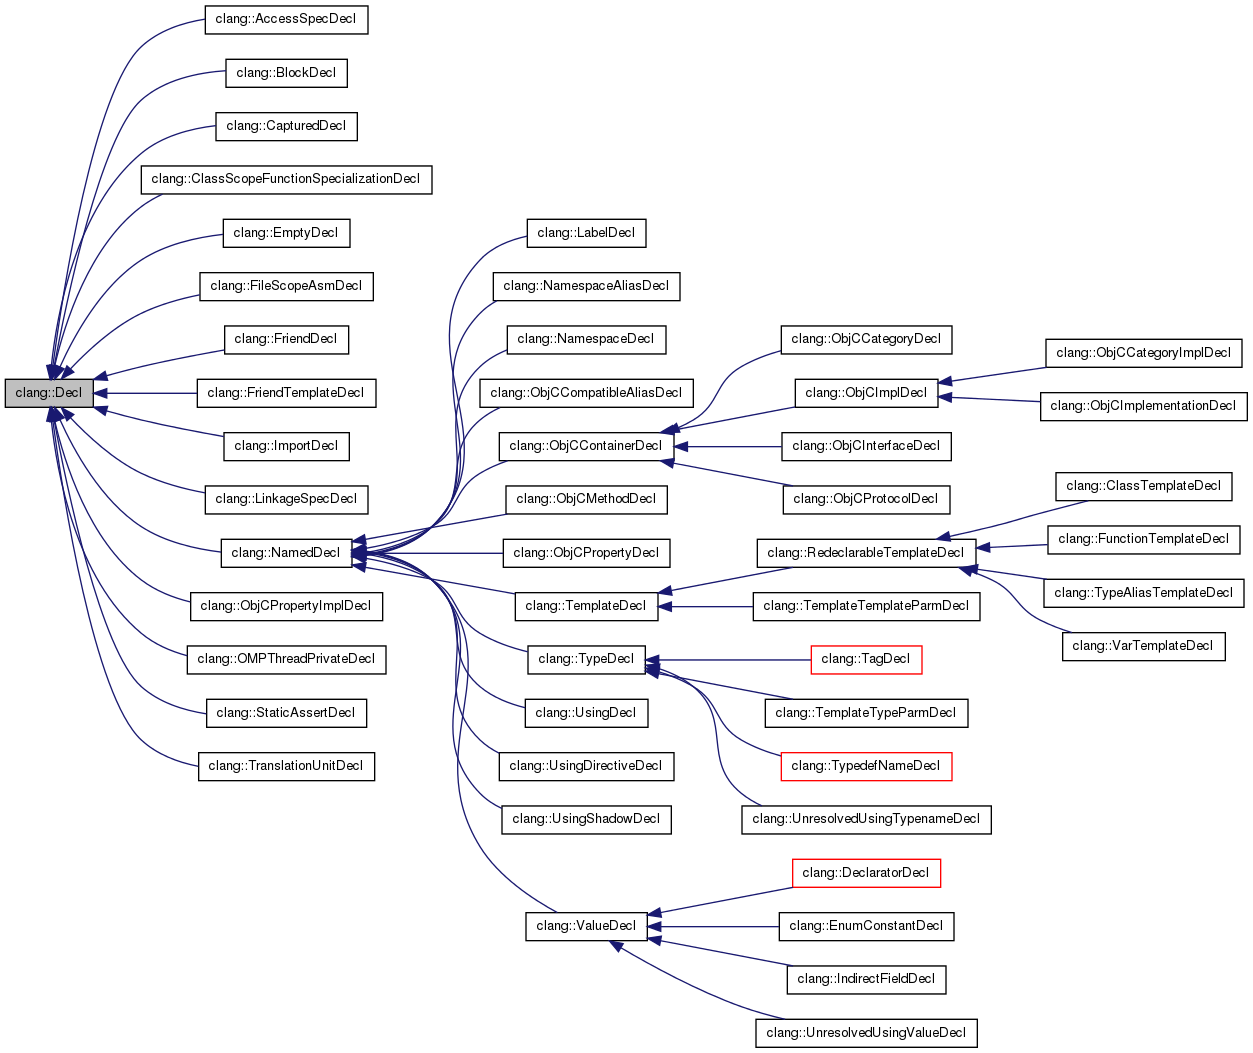
\includegraphics[height=.8\textheight]{figures/decl-hierarchy}
\end{frame}

\begin{frame}
  \frametitle{AST of helloworld prog}
  %% \only<1>{\lstinputlisting[language=c]{listings/helloworld.c}}
  %% \only<2>{\lstinputlisting{listings/helloworld.ast}}
  \lstinputlisting[language=c]{listings/helloworld.c}
  \centerline{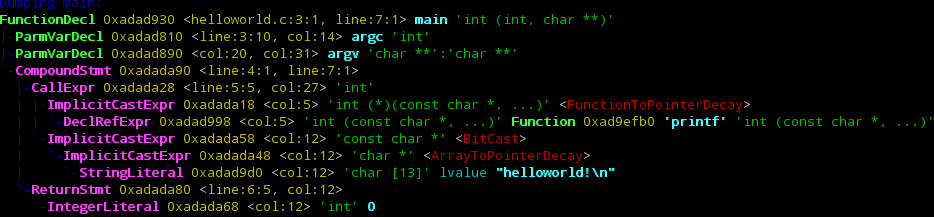
\includegraphics[width=\textwidth]{figures/helloworld}}
\end{frame}

%% \begin{frame}
%%   \frametitle{Important AST classes}
%%   \begin{itemize}
%%     \item TranslationUnitDecl
%%     \item ASTContext
%%   \end{itemize}
%% \end{frame}

\section{Structure of Clang tools}
\frame{\tableofcontents[currentsection]}
\begin{frame}
  \frametitle{Important datatypes}
  \begin{itemize}
    \item ClangTool, RefactoringTool
    \item ToolAction, FrontendActionFactory
    \item FrontendAction
    \item ASTConsumer
    \item RecursiveASTVisitor
  \end{itemize}
\end{frame}

\begin{frame}
  \frametitle{Typical design of Clang tools}
  \centerline{\includegraphics[width=.8\textwidth]{figures/clangtool-structure}}
\end{frame}

\begin{frame}
  \frametitle{RecursiveASTVisitor<...>}
  The \texttt{RecursiveASTVisitor<...>} class, which provides 3 kinds of APIs,
  is the main interface to manipulate Clang AST.
  \begin{itemize}
    \item \texttt{Traverse*} methods
    \item \texttt{WalkUpFrom*} methods
    \item \texttt{Visit*} methods
  \end{itemize}
\end{frame}

\begin{frame}
  \frametitle{RecursiveASTVisitor's visiting scheme}
  \begin{itemize}
    \item \texttt{Traverse*} the AST using depth first order
    \item At each node, \texttt{WalkUpFrom*} its inheritance hierarchy
    \item For each class, call \texttt{Visit*}
  \end{itemize}
  \pause
    \centerline{\includegraphics[height=.4\textheight]{figures/visiting-scheme}}
  \pause
  \alert{Just subclass \texttt{RecursiveASTVisitor}
    and override methods related to the AST nodes you concern!}
\end{frame}

\begin{frame}
  \frametitle{A visitor example}
  Dump all enum declarations in namespace \texttt{NS}
  %% \lstinputlisting[language=C++]{listings/myvisitor.cpp}
  \begin{figure}
    \centerline{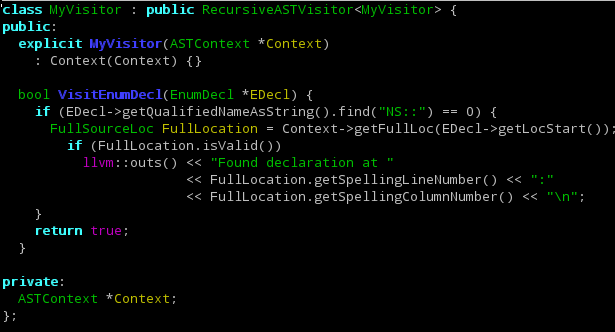
\includegraphics[width=\textwidth]{figures/myvisitor}}
  \end{figure}
\end{frame}

\section{AST Matcher library}
\frame{\tableofcontents[currentsection]}
\begin{frame}
  \frametitle{The AST Matcher library}
  Clang AST Matcher library support filtering the AST using specified
  ``filters'', say, matchers.
  \pause
  \begin{block}{examples}
    \begin{itemize}
    \item \texttt{functionDecl(hasAnyParameter(anything))}
    \item \texttt{recordDecl(hasMethod(hasName("foo")))}
    \end{itemize}
  \end{block}
\end{frame}

\begin{frame}
  \frametitle{Bind matchers to names}
  Names can be bound to matchers, enabling you to retrieval matched nodes.
  \begin{figure}
    \centerline{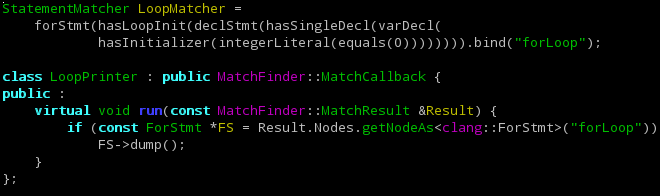
\includegraphics[width=\textwidth]{figures/matcherbind.png}}
  \end{figure}
\end{frame}

\begin{frame}
  \frametitle{How matchers work?}
  Using the \texttt{MatchFinder} class.
  \begin{itemize}
    \item<1-> \texttt{void addMatcher(Matcher<...>\&, MatchCallBack*)}\\
      Register a matcher object with a callback object,
      overloaded for all six AST node types (recall)
    \item<2-> \texttt{MatchFinder::MatchResult}\\
      Containing infomation of matched AST nodes.
    \item<3-> \texttt{MatchFinder::MatchCallBack}\\
      \texttt{void MatchCallBack::run(MatchResult\&)}\\
      Inner class with a \texttt{run} method. Every time a match is found,
      The \texttt{MatchFinder} will invoke the registered \texttt{MatchCallBack} object,
      passing it a \texttt{MatchResult} object
  \end{itemize}
\end{frame}

\begin{frame}
  \frametitle{Inject matchers into Clang Tool structure}
  The \texttt{MatchFinder} class defines the \texttt{newASTConsumer} method,
  so we can create a \texttt{FrontendActionFactory} object with a \texttt{MatchFinder} object.
  \pause
  \begin{figure}
    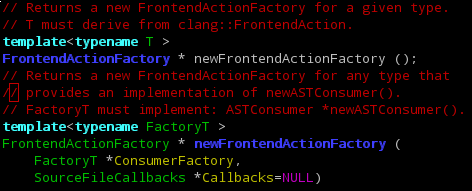
\includegraphics[width=.8\textwidth]{figures/createfrontendfactory}
  \end{figure}
  \pause
  \alert{\texttt{MatchFinder} is yet another kind of \texttt{FrontendAction}!}
\end{frame}

\begin{frame}
  \frametitle{Recall: typical design of Clang tools}
  \centerline{\includegraphics[width=.8\textwidth]{figures/clangtool-structure}}
\end{frame}

\begin{frame}
  \frametitle{A real-world example}
  \centerline{The \alert{clang-check} tool}
\end{frame}

\section{Summary}
\frame{\tableofcontents[currentsection]}
\begin{frame}
  \frametitle{Summary}
  \begin{itemize}
    \item<1-> The Clang AST\\
      6 node types, among which \texttt{Decl, Stmt, Type are the most important},
      each forms a class hierarchy.
    \item<2-> Structure of Class tool\\
      Several important classes, hooked up one by one
    \item<3-> AST Matcher library\\
      Find what you want, and easily injected into general Clang tools' structure
  \end{itemize}
\end{frame}

\begin{frame}
  \frametitle{References}
  \begin{itemize}
    \item http://clang.llvm.org/docs/index.html
    \item http://clang.llvm.org/docs/LibASTMatchers.html
    \item https://github.com/loarabia/Clang-tutorial
  \end{itemize}
\end{frame}

\frame{\centerline{\Huge the end}}

\end{document}
